\section{VC Dimension}
\label{sec:vc-dimension}
\begin{enumerate}
\item ~[5 points] Assume that the three points below can be labeled
  in any way.  Show with pictures how they can be shattered by a
  linear classifier.  Use filled dots to represent positive classes
  and unfilled dots to represent negative classes.


  \begin{tikzpicture}
    \begin{axis}[my style, xtick={-1,0,...,3}, ytick={-1,0,...,3},
      xmin=-1, xmax=3, ymin=-1, ymax=3]
      \addplot[mark=*,only marks] coordinates {(2,2)(1,1)(1,2)};
    \end{axis}
  \end{tikzpicture}
\begin{solution}

\begin{tikzpicture}
    \begin{axis}[my style, xtick={-1,0,...,3}, ytick={-1,0,...,3},
      xmin=-1, xmax=3, ymin=-1, ymax=3]
      \addplot[mark=*,only marks] coordinates {(2,2)(1,1)(1,2)};
      \addplot [domain=-10:10, samples=2] {x-1};
    \end{axis}
 \end{tikzpicture}
 \hspace{1cm}
 \begin{tikzpicture}
    \begin{axis}[my style, xtick={-1,0,...,3}, ytick={-1,0,...,3},
      xmin=-1, xmax=3, ymin=-1, ymax=3]
      \addplot[mark=o,only marks] coordinates {(2,2)(1,1)(1,2)};
      \addplot [domain=-10:10, samples=2] {x-1};
    \end{axis}
 \end{tikzpicture}
 \hspace{1cm}
 \begin{tikzpicture}
    \begin{axis}[my style, xtick={-1,0,...,3}, ytick={-1,0,...,3},
      xmin=-1, xmax=3, ymin=-1, ymax=3]
      \addplot[mark=o,only marks] coordinates {(1,1)(1,2)};
      \addplot[mark=*,only marks] coordinates {(2,2)};
      \addplot [domain=-10:10, samples=2] (1.5,x);
    \end{axis}
 \end{tikzpicture}
 \hspace{1cm}
 \begin{tikzpicture}
    \begin{axis}[my style, xtick={-1,0,...,3}, ytick={-1,0,...,3},
      xmin=-1, xmax=3, ymin=-1, ymax=3]
      \addplot[mark=*,only marks] coordinates {(1,1)(1,2)};
      \addplot[mark=o,only marks] coordinates {(2,2)};
      \addplot [domain=-10:10, samples=2] (1.5,x);
    \end{axis}
 \end{tikzpicture}
 \hspace{1cm}
 \begin{tikzpicture}
    \begin{axis}[my style, xtick={-1,0,...,3}, ytick={-1,0,...,3},
      xmin=-1, xmax=3, ymin=-1, ymax=3]
      \addplot[mark=o,only marks] coordinates {(2,2)(1,1)};
      \addplot[mark=*,only marks] coordinates {(1,2)};
      \addplot [domain=-10:10, samples=2] {x+0.5};
    \end{axis}
 \end{tikzpicture}
 \hspace{1cm}
 \begin{tikzpicture}
    \begin{axis}[my style, xtick={-1,0,...,3}, ytick={-1,0,...,3},
      xmin=-1, xmax=3, ymin=-1, ymax=3]
      \addplot[mark=*,only marks] coordinates {(2,2)(1,1)};
      \addplot[mark=o,only marks] coordinates {(1,2)};
      \addplot [domain=-10:10, samples=2] {x+0.5};
    \end{axis}
 \end{tikzpicture}
  \hspace{1cm}
 \begin{tikzpicture}
    \begin{axis}[my style, xtick={-1,0,...,3}, ytick={-1,0,...,3},
      xmin=-1, xmax=3, ymin=-1, ymax=3]
      \addplot[mark=*,only marks] coordinates {(1,2)(2,2)};
      \addplot[mark=o,only marks] coordinates {(1,1)};
      \addplot [domain=-10:10, samples=2] (x,1.5);
    \end{axis}
 \end{tikzpicture}
 \hspace{1cm}
 \begin{tikzpicture}
    \begin{axis}[my style, xtick={-1,0,...,3}, ytick={-1,0,...,3},
      xmin=-1, xmax=3, ymin=-1, ymax=3]
      \addplot[mark=o,only marks] coordinates {(1,2)(2,2)};
      \addplot[mark=*,only marks] coordinates {(1,1)};
      \addplot [domain=-10:10, samples=2] (x,1.5);
    \end{axis}
 \end{tikzpicture}
\end{solution}
\item {\bf VC-dimension of axis aligned rectangles in $\mathbb{R}^d$}:
  Let $H^d_{rec}$ be the class of axis-aligned rectangles in
  $\mathbb{R}^d$. When $d=2$, this class simply consists of rectangles
  on the plane, and labels all points strictly outside the rectangle
  as negative and all points on or inside the rectangle as positive.
  In higher dimensions, this generalizes to $d$-dimensional boxes,
  with points outside the box labeled negative.

  \begin{enumerate}
  \item ~[10 points] Show that the VC dimension of $H^2_{rec}$ is 4.
  \begin{figure}[!htbp]
  \begin{center}
	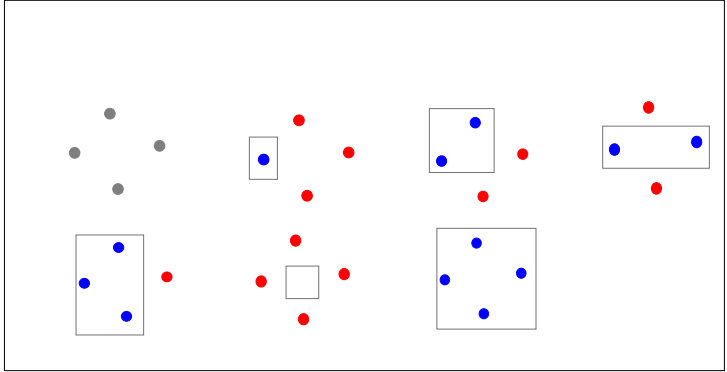
\includegraphics[width=.5\linewidth]{auto/Capture}
	\caption{Shattering of 4 points for axis aligned rectangles}
	\end{center}
	\end{figure}
  \begin{solution}
  If we take any four points randomly or on the corners of the rectangle, the adversary can label them in such a way that they will not be shatterable. So we will take a points on the edges. As we can see in the figure the points are shatterble. In case of $5$ points , our adversary can always label them in such a way that the points will never be shatterable. Therefore the VC dimension of $H^2_{rec}$ is 4.
  
  \end{solution}
  \item ~[10 poin
  ts] Generalize your argument from the previous proof
    to show that for $d$ dimensions, the VC dimension of $H^d_{rec}$
    is $2d$.
    \begin{solution}
    Using the above explanation we can see that for a 2 - dimensional of axis aligned rectangles the VC dimension was 4. This is equal to 2 times the dimensional. For an extra point there is always a point which is either inside the rectangle or is marked negative, which cannot be consistent with the axis aligned rectangles. Using the same general understanding for higher dimension we can conclude that  for d dimensions, the VC dimension of $H^d_{rec}$ is 2d.
    \end{solution}
  \end{enumerate}
  
\item In the lectures, we considered the VC dimensions of infinite
  concept classes. However, the same argument can be applied to finite
  concept classes too. In this question, we will explore this setting.

  \begin{enumerate}
  \item ~[10 points] Show that for a finite hypothesis class
    $\mathcal{C}$, its VC dimension can be at most
    $\log_2\left(|\mathcal{C}|\right)$. (Hint: You can use
    contradiction for this proof. But not necessarily!)
\begin{solution}
Considering that for a finite hypothesis class $\mathcal{C}$, its VC($\mathcal{C}$) $=$ d. As there are d points we can label them in $2^d$ ways.

The $2^d$ combinations can be in worst case classified by the size of entire hypothesis class $|\mathcal{C}|$. Therefore $2^d \leq |\mathcal{C}|$ .
Taking log on both side we get $d \leq \log_2\left(|\mathcal{C}|\right)$.
\end{solution}
  \item ~[5 points] Find an example of a class $\mathcal{C}$ of
    functions over the real interval $X = [0,1]$ such that
    $\mathcal{C}$ is an {\bf infinite} set, while its VC dimension is
    exactly one.
\begin{solution}
For a class of function over the real interval $X = [0,1]$ is a left bounded interval $[0,a)$ in it. Here we can see that the function $f(x) = +1 if 0 \leq x < a$  defines the infinite set. We know that for this the VC dimension is 1.
\end{solution}
  \item ~[5 points] Give an example of a {\bf finite} class
    $\mathcal{C}$ of functions over the same domain $X = [0,1]$ whose
    VC dimension is exactly $\log_2(|\mathcal{C}|)$.
\begin{solution}
We can see that over the same domain $X = [0,1]$ a finite class $\mathcal{C}$ is a function of Integers. Hence, we can deduce the class as $[0,1]$ where the function can either be positive for value $x=1$ or value $x=0$. There fore there are 2 functions. But only one of them is shatterable, which is VC = $\log_2 (2) = 1$. Hence VC dimension for it is exactly $\log_2(|\mathcal{C}|)$.
\end{solution}
  \end{enumerate}
  
\end{enumerate}

%%% Local Variables:
%%% mode: latex
%%% TeX-master: "hw3"
%%% End:
